\documentclass[11pt]{llncs}
\usepackage{graphicx}
\usepackage{url}
\usepackage{hyperref}
\usepackage{fontspec}
\usepackage{float}

\setmainfont{Carlito} % Open-source Calibri alternative

\begin{document}

\title{A Study of \textit{Enhancing Hand--Object Interactions in Virtual Reality for Precision Manual Tasks}}
\author{William C. Bogdanovic \and Théo L. Hyvert}
\institute{M2 SIS, Gaspard-Monge Institute, Gustave Eiffel Campus, FRANCE}
\maketitle

\section*{Introduction}
Despite the rapid evolution of Virtual Reality (VR) hardware and visual rendering, enabling truly natural, precise hand--object interactions remains a persistent challenge. Conventional methods often rely on over-simplified hand models or purely physics-based systems, which either fail to capture realistic finger coordination or become computationally heavy for real-time performance. In \emph{Enhancing Hand--Object Interactions in Virtual Reality for Precision Manual Tasks} (Mangalam et al.\ 2024), the authors propose a bio-inspired framework informed by biomechanics, neuroscience, and psychophysics. They argue that \emph{synergy-based} hand modeling, paired with adaptive collision handling, can create more realistic and efficient VR environments, especially for applications that require fine motor skills (such as precise object assembly or surgical training).

\vspace{1em}
\noindent
\textbf{Technological and Cognitive Motivations.} The technological motivation stems from a need to simulate not just visually convincing but \emph{functionally accurate} hand interactions, which can be complex given the hand's many joints and real-world collision dynamics. On the cognitive side, the paper points out that fluid manipulation depends on the user's sense of ownership over their virtual hand, as well as accurate anticipation of collision forces (e.g., knowing where and when an object is ``in grasp'').

The hands have a very delicate and complex structure. Composed of a network of bones, nerves, and around $10 \%$ of all the muscles of a human body, computing the interaction of the user's hands can be a daunting task.
How can the user tell the material of an object? If it is slippery, how can he know that his virtual hand are applying enough pressure to prevent the object from falling down. Since people are used to their body that they trained on all their life, having a new pair of hands can be like discovering a new limb, and due to muscular memory, it can be frustrating to be clumsy with your own hands.

By aligning the control parameters of the virtual hand with known psychophysical constraints (like digit synergies), the approach can meet both technological performance goals (fast, real-time simulation) and cognitive realism (intuitive user experience).

\section*{Key Contributions and Thematic Overview}
\paragraph{Synergy-Based Modeling of the Virtual Hand.}
Human fingers often move in coordinated patterns called ``synergies,'' which drastically reduce the effective degrees of freedom needed for common grasps. The authors capitalize on this by limiting the virtual hand’s motion to these principal components, thereby decreasing computation while preserving realism. This synergy-based approach particularly benefits time-critical tasks like in-assembly VR or laparoscopic surgery simulations, where reaction time and coordination are paramount.

\paragraph{Collision Handling \& Bio-Inspired Insights.}
Another pivotal focus is collision detection and response. Purely heuristic solutions typically fail when encountering novel objects or unforeseen finger placements, whereas purely physics-based approaches can slow down or become unstable. The paper’s hybrid solution uses simplified heuristics to launch a stable grasp, but once contact is established, physics-based micro-corrections refine the final grip. This avoids heavy computations at every instant, yet prevents the abrupt ``snapping'' or unnatural interpenetration often reported in simpler methods.

\paragraph{Experimental Tasks and Measures.}
Participants carried out tasks such as lifting and rotating small virtual blocks, assembling mechanical parts, and fine in-hand manipulations. Critically, the researchers measured:
\begin{itemize}
    \item \textbf{Completion time:} How long participants took to accomplish each task.
    \item \textbf{Error rates:} Incidents of slippage, failed grasp, or object misplacement.
    \item \textbf{Subjective feedback:} Presence, ownership, and perceived agency via standard questionnaires.
\end{itemize}
Their findings suggest that synergy-based models plus adaptive collision handling reduce unintended finger--object interpenetrations and yield smoother, more intuitive interactions.

\begin{figure}[H]
\centering
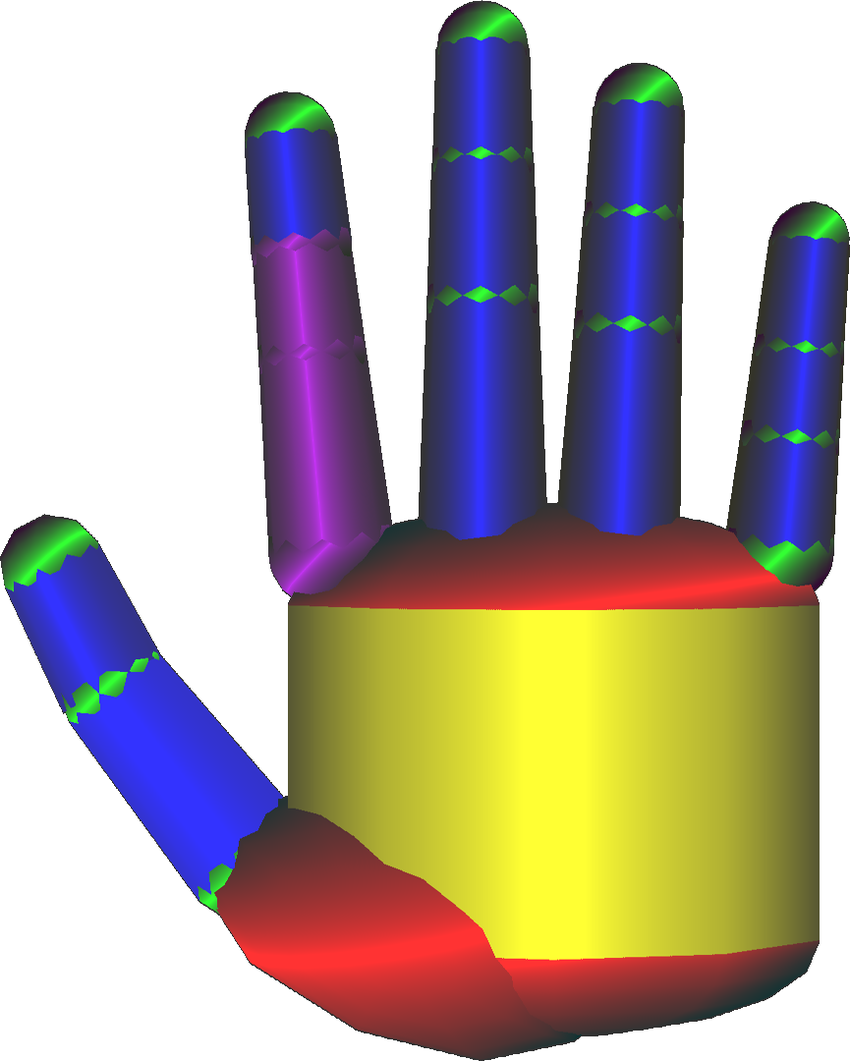
\includegraphics[width=0.25\textwidth]{synergy-based_hand_model.png}
\caption{The figure above shows a 3D synergy-based hand model used for pose reconstruction. The differently color-coded phalanges highlight the different anatomical segmentations and movement constraints. The purple segment marks the proximal interphalangeal joint of the index finger, and its different color emphasizing its unique role in independent articulation. Other fingers remain in a neutral state, showing their relative positioning, adapted from \cite{Ciotti2016}. The distinct colors indicate synergy groups derived from various hand postures, suggesting that the blue-colored portions experience constrained movement, allowing for a simplified representation of joint mobility.}
\label{fig:synergy-model}
\end{figure}

\section*{Technologies and Interaction Techniques}
\paragraph{Display and Input Devices.}
While the paper does not lock onto one specific commercial headset, the authors emphasize modern VR head-mounted displays (e.g., devices with high frame rates and inside-out tracking) to maintain user immersion. Optical or controller-based hand-tracking approaches (like Leap Motion, or built-in cameras on consumer VR headsets) feed real-time pose data into the synergy-based engine.

\paragraph{Tracking Systems and Data Flow.}
The synergy framework can leverage multiple sensor inputs: standard controller orientation, or more advanced finger tracking if available. The authors note that data gloves could also be used, but many remain bulky. They stress a need for calibration to ensure each user's real-hand posture properly maps to the synergy-based hand avatar—especially important for high-precision tasks.

\paragraph{Interaction Design.}
Interaction techniques revolve around direct hand manipulation: users attempt to grab the virtual object using their natural finger closure. The system detects collision initiation through heuristics (e.g., contact points or bounding volumes). Then, once a grasp is deemed stable, local physics-based corrections anchor the object to the hand. This two-step approach balances real-time efficiency (no full physics at all times) and accuracy (no floating objects).

\begin{figure}[H]
\centering
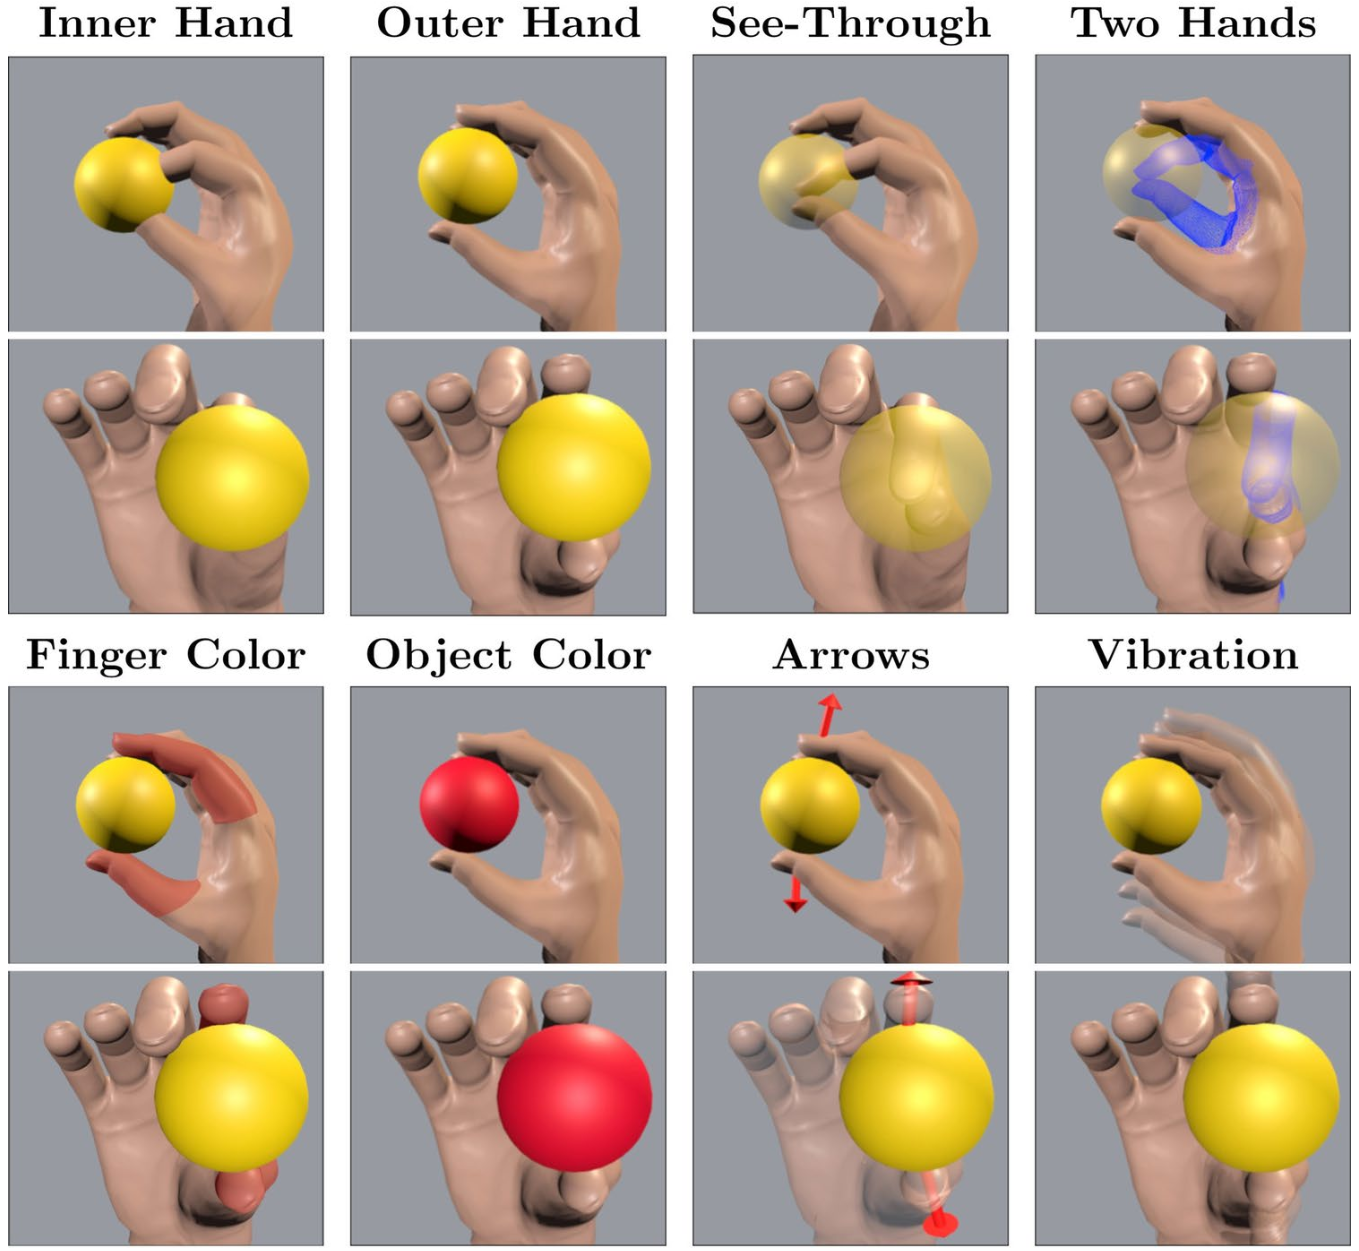
\includegraphics[width=0.75\textwidth]{Virtual Hand-Object.png}
\caption{The figure above from \cite{Mangalam2024} shows the different methods that can be used to show to the user the current state of his hands. Going from simple visual cues such as changing the object color to changing the object opacity or clamping the fingers positions to the boundary of the object.}
\label{fig:virtual-hands}
\end{figure}

\section*{Bio-Inspired Framework in Detail}
\paragraph{Neuroscience and Psychophysics Underpinnings.}
Real grasping is highly sensitive to multisensory feedback, including digit coordination and subtle force adjustments. By embedding synergy constraints, the authors replicate natural finger interplay. This fosters a stronger sense of embodiment, because the user subconsciously recognizes that the virtual hand’s shape changes match their internal motor patterns. Beyond performance, the approach addresses cognitive demands by lowering the mental dissonance between what the user intends and what they see.

\paragraph{Local vs.\ Global Constraints.}
The authors highlight that synergy patterns can preserve ``global'' hand shape with only local, simplified checks. Rather than testing every finger joint in real time, synergy-based constraints act as a strong prior---they ensure that if the index finger flexes, for example, the middle finger might subtly follow without needing an expensive collision check for each millimeter of motion. This speeds up computations and reduces glitchy motions.

\paragraph{Advances in Release Mechanics.}
An especially frequent complaint in VR is the \emph{awkward release}: objects may pop out of the user’s hand or require exaggerated finger splaying. Here, a modest allowance for intersection between hand and object helps maintain a believable continuity of motion. The authors found that letting the virtual fingertips partially occupy the object’s boundary—just during the release transition—cuts down user frustration and fosters a more realistic letting-go experience.

\section*{Methodological Critique and Proposed Improvements}
One limitation is that most of the paper’s experiments involved small, rigid shapes. While synergy-based constraints show promise, future work should address \emph{deformable} or multi-part objects (like cloth or a puzzle with interlocking pieces). Additionally, the study does not deeply discuss sample size or prior user experience with VR. A broader user group, possibly novices vs.\ experts, might reveal subtle differences in how synergy-based interactions affect error rates and presence.

Furthermore, the authors rely mainly on self-report measures (presence, ownership). These metrics are standard, but deeper \emph{longitudinal} or real-to-virtual skill-transfer studies would better assess the system's true training benefits. Another methodological concern is the lack of direct haptic feedback. The synergy approach masks some unnatural collisions, but truly faithful manipulation may still need tactile cues. To mitigate potential confounds, an improved design could:
\begin{itemize}
    \item Include a larger participant pool (both VR veterans and newcomers).
    \item Compare synergy-based modeling against a purely physics-based baseline on the same tasks.
    \item Introduce a simple wearable vibrotactile device to test if partial haptic feedback further reduces error.
\end{itemize}
By systematically evaluating these modifications, we can see whether synergy constraints alone suffice or if they must be paired with specialized feedback for more advanced tasks.

\section*{Discussion and Future Directions}
\paragraph{Scalability \& Parallelization.}
The synergy approach can lessen CPU load, but tasks with multiple simultaneous grasps or complex geometry may still push performance limits. The authors suggest parallelizing synergy and collision checks on GPUs or multi-core systems. This could keep latencies low, especially for multi-handed interactions or collaborative VR sessions.

\paragraph{Haptic Feedback Potential.}
While synergy-based modeling partially compensates for absent force feedback (by preventing overt visual errors), rich haptic cues might further enhance realism. Light gloves or ultrasonic arrays could convey contact points or friction. This synergy-haptic blend may yield better user acceptance in high-precision scenarios like medical VR. Moreover, analyzing with said gloves the most frequent movements of a surgical operation to focus on the most import contact points could make the computation faster.

\paragraph{Object Diversity.}
Most examples center on small, rigid items. Extending synergy-based constraints to objects with unusual mass distributions, or squishy surfaces, remains an open question. The authors propose an adaptive synergy matrix that modifies how each finger synergy responds to dynamic shape deformations, but this requires more research.

\paragraph{User-Centric Validation.}
Finally, longer and more natural tasks---like virtual assembly lines or actual surgical sub-procedures---would demonstrate the framework's applicability. Over time, we could measure whether synergy-based VR fosters better skill retention or cross-domain motor training. This addresses a key cognitive perspective: does synergy-based modeling lighten users' mental workload, enabling them to focus on complex tasks rather than wrestling with unrealistic finger constraints?

\section*{Conclusion}
\emph{Enhancing Hand--Object Interactions in Virtual Reality for Precision Manual Tasks} (Mangalam et al.\ 2024) offers a robust demonstration that synergy-based virtual hand models, combined with adaptive collision handling, can significantly improve VR realism and user experience. By weaving together ideas from biomechanics (digit synergies), neuroscience (feedback loops, embodiment), and computer science (hybrid collision detection), the authors alleviate two common complaints: unnatural penetration and ``snappy'' release. Although future work is needed to confirm generalizability---especially for non-rigid or large-scale objects, haptic integration, and broader participant groups---the paper’s results indicate that synergy-based methods can handle many of the intricate demands of precision tasks in VR. This approach thus provides a promising pathway for both technological refinements (faster, more stable simulation) and cognitive benefits (enhanced presence, reduced user frustration).

\vspace{1em}
\noindent

\begin{thebibliography}{1}

\bibitem{Mangalam2024}
M. Mangalam, S. Oruganti, G. Buckingham, C. W. Borst,
``Enhancing hand-object interactions in virtual reality for precision manual tasks,''
\textit{Virtual Reality},
vol. 28, no. 166, 2024.
\url{https://doi.org/10.1007/s10055-024-01055-3}.

\bibitem{Ciotti2016}
S. Ciotti, E. Battaglia, I. Oikonomidis, M. Bianchi,
``Synergy-driven Performance Enhancement of Vision-based 3D Hand Pose Reconstruction,''
Conference Paper, Nov. 2016.
% \url{https://www.researchgate.net/publication/309476562_Synergy-driven_Performance_Enhancement_of_Vision-based_3D_Hand_Pose_Reconstruction}
\url{https://users.ics.forth.gr/~argyros/mypapers/2016_11_MobiHealth_synergies.pdf}

\end{thebibliography}

\end{document}